\documentclass{cheatsheet}
\usepackage{bm}
\usepackage{textcomp, mathcomp}
\usepackage{empheq}
\usepackage{pbox}

\doctitle{Chemistry Cheatsheet}
\author{Noa Sendlhofer \& Christian Leser \\ nsendlhofer \& cleser}

\begin{document}
\section{1. Basics} %Noa
	\subsection{1.1 Unit conversions}
	\begin{itemize}
		\itemsep0em
		\raggedright
  		\item \textbf{Energy:} $1eV=1.602\cdot 10^{-19}J$,    $1cal=4.18J$
    	\item \textbf{Pressure:} $P = \frac{F}{A} = \rho \cdot h \cdot g$\\ $1 \textrm{atm} = 760mm \; \textrm{Hg} = 760 \textrm{torr} = 101'325 \textrm{Pa} = 1.01325 \textrm{bar}$\\ Manometer: $P = P_{atm}\pm \rho g h$
    	\item \textbf{Force:} $F = m \cdot g, \; m = \rho \cdot V$
		\item \textbf{Amount of substance:} $1 \textrm{mol} = 6.022\cdot 10^{23} \textrm{(Avogadro)}$
    	\item \textbf{Length:} $1\text{Å}=10^{-10}m$
    	\item \textbf{STP; } $0\tccentigrade = 273.15K, \; 1atm; \; V_m = 22.41L$
	\end{itemize}

\subsection{1.2 General}
    \begin{itemize}
		\itemsep0em
        \item \textbf{Kinetic energy:} $E_{kin} = \frac{1}{2} \cdot m \cdot v^2$
        \item \textbf{Potential energy:} $E_{pot} = m \cdot g \cdot \Delta h$
        \item \textbf{electrostatic:} $E_{el}=\frac{\kappa Q_1Q_2}{d^2}$\quad $\kappa = \frac{1}{4\pi \epsilon_0}$
        \item \textbf{Photon energy: } $E_\gamma = h\cdot f = \frac{h\cdot c}{\lambda}$
        \item \textbf{De Broglie wavelength: } $\lambda = \frac{h}{m\cdot v}$
    \end{itemize}
    	
\subsection{1.3 Trends in the periodic table of elements}
	\begin{itemize}
		\itemsep0em
    	\item \textbf{Ionisation energy: }The ionization energy is the quantity of energy that an isolated, gaseous atom in the ground electronic state must absorb to discharge an electron, resulting in a cation.
    	\item \textbf{Electron affinity: }Electron affinity is defined as the change in energy (in kJ/mole) of a neutral atom (in the gaseous phase) when an electron is added to the atom to form a negative ion.
    	\item \textbf{Electronnegativity:} Electronegativity is a measure of an atom's ability to attract shared electrons to itself.
	\end{itemize}
	\centerline{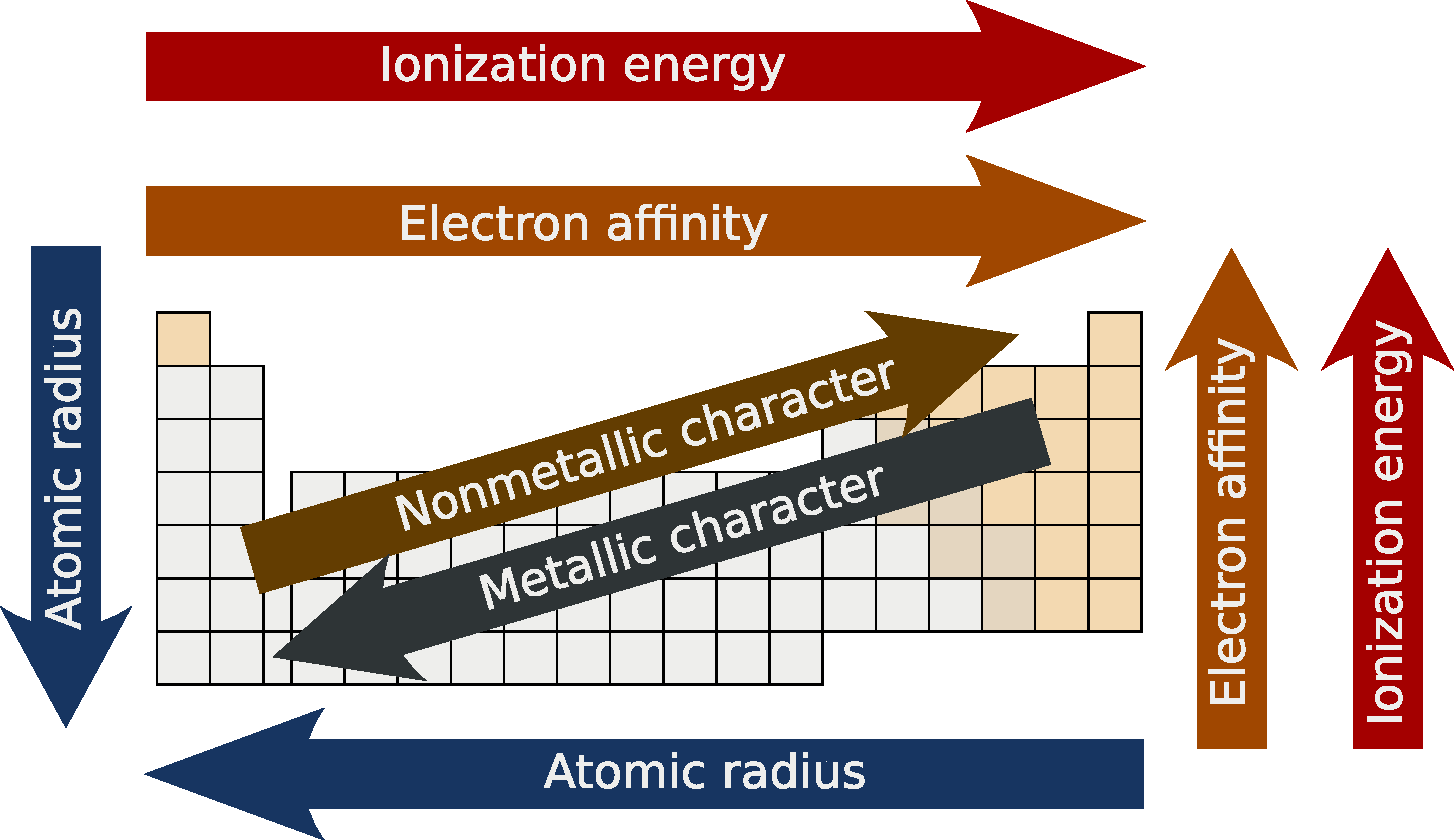
\includegraphics[width=0.65\linewidth]{src/1_Basics/Periodic_trends.pdf}}
	\vspace*{0.5em}

\section{2. Atoms} %Christian
	\subsection{2.1 Quantum mechanics}
    \begin{scriptsize}
        \begin{tabular}{c c}
            Atomic mass = total mass & Atomic weight = average atomic mass (isotopes)\\
            Atomic number = \#protons & mass number = \#protons + \#neutrons
        \end{tabular}
    \end{scriptsize}
        \vspace*{0.0em}
        
        Heisenbergs uncertainty principle $\Delta x \cdot \Delta p \geq \frac{h}{4 \cdot \pi}$ Due to duality of electrons (acting like waves and elementary entities at the same time), impossible to exactly describe position and momentum simultaneously.\\
        \textbf{Effective nuclear charge (approx.):}   $Z_{eff} = Z-S$\\
        $Z$ = \#protons, $S$ = \#$e^-$ on all full shells
        \vspace{1mm}\\
        In periodic table: $Z_{eff}$ increases from left to right $\rightarrow$ electrons are more attracted and hence atomic radius is smaller, the further right in the periodic table. ($e^-$ repulsion vs. nuclear charge)
        \vspace*{0.0em}
	\subsection{2.2 Orbitals}
  \begin{minipage}{0.99\linewidth}
    \begin{minipage}{0.33\linewidth}
      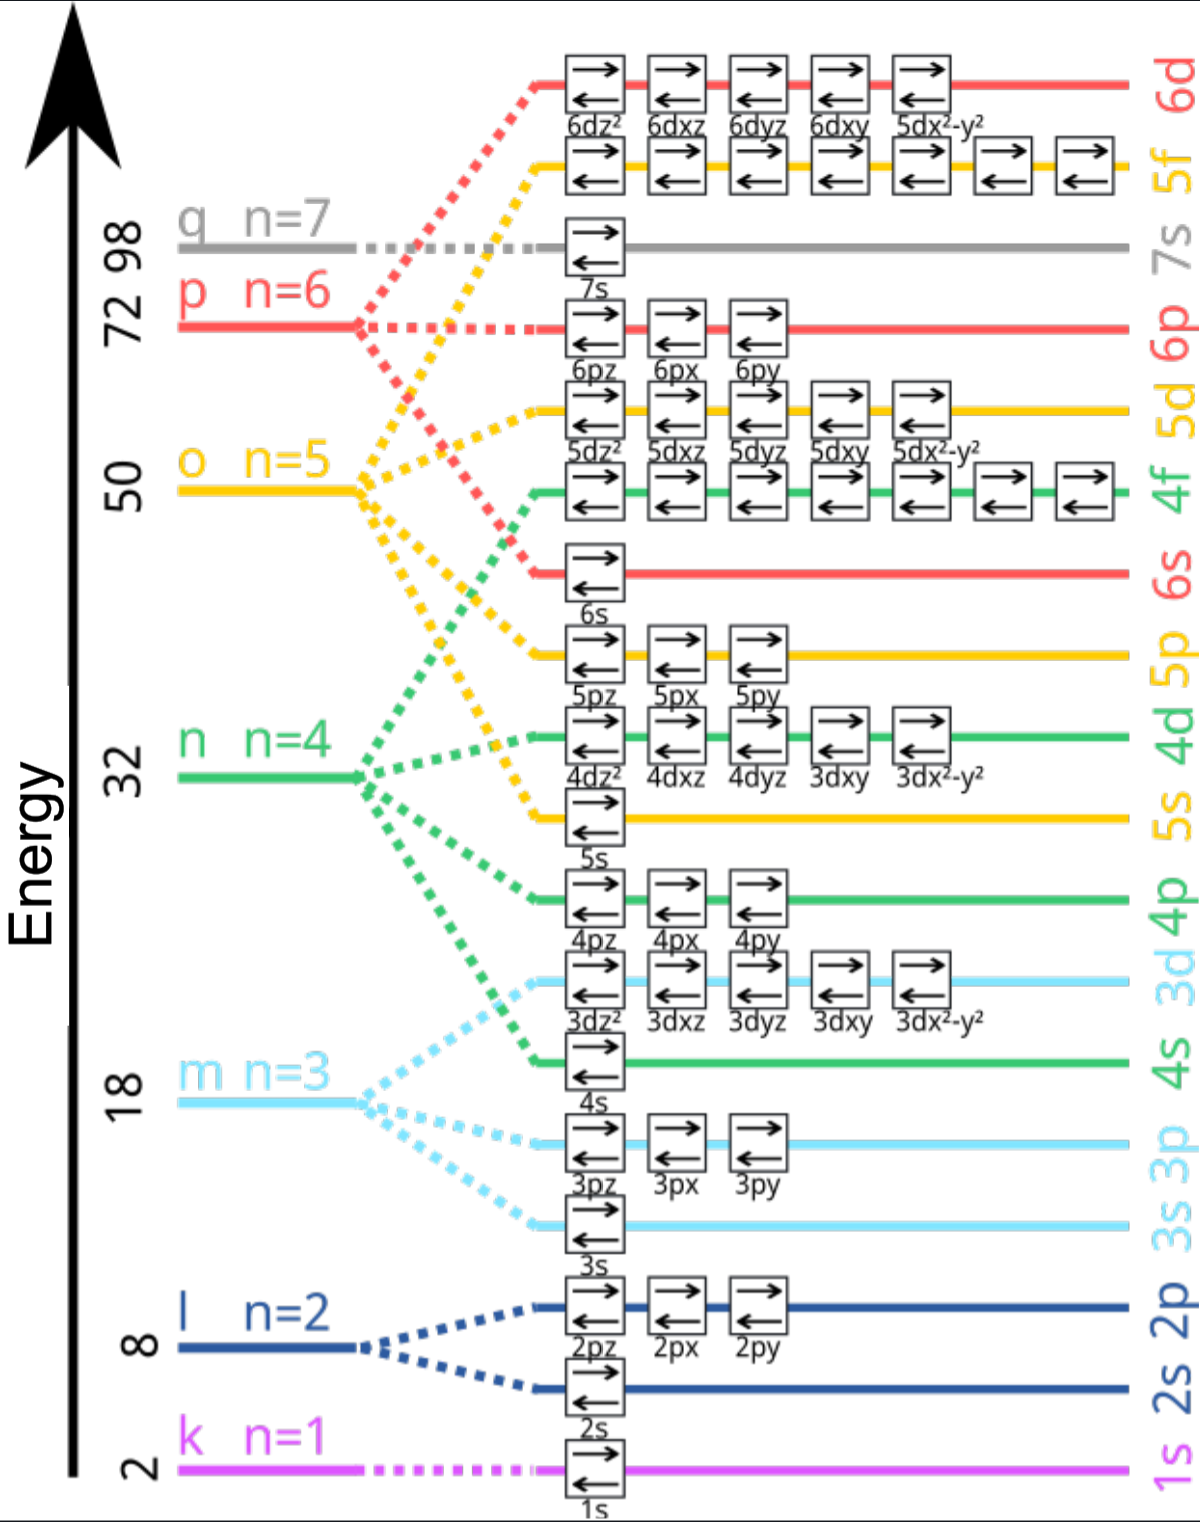
\includegraphics[width = 2.3cm]{src/2_Atoms/images/Energieniveau.png}
    \end{minipage}
    \begin{minipage}{0.52\linewidth}
      \begin{scriptsize}
        \begin{center}
            \begin{tabular}{|p{0.3mm}|c|p{0.07\textwidth}|c|c|}
                \multicolumn{1}{p{0.3mm}}{n} & \multicolumn{1}{c}{l} & \multicolumn{1}{p{0.07\textwidth}}{\rotatebox{90}{\pbox{1.5cm}{subshell\\ designation}}} & \multicolumn{1}{c}{$m_i$} & \multicolumn{1}{c}{$m_s$} \\ [0.5ex]
                \hline
                1 & 0, s & 1s                                  & 0                      & $\pm 1/2$ \\ 
                \hline
                2 & 0, s & 2s                                  & 0                      & $\pm 1/2$ \\
                  & 1, p & 2p                                  & 1, 0, -1               & $\pm 1/2$ \\
                \hline
                3 & 0, s & 3s                                  & 0                      & $\pm 1/2$ \\
                  & 1, p & 3p                                  & 1, 0, -1               & $\pm 1/2$ \\
                  & 2, d & 3d                                  & 2, 1, 0, -1, -2        & $\pm 1/2$ \\
                \hline
                4 & 0, s & 4s                                  & 0                      & $\pm 1/2$ \\
                  & 1, p & 4p                                  & 1, 0, -1               & $\pm 1/2$ \\
                  & 2, d & 4d                                  & 2, 1, 0, -1, -2        & $\pm 1/2$ \\
                  & 3, f & 4f                                  & 3, 2, 1, 0, -1, -2, -3 & $\pm 1/2$ \\
                \hline
            \end{tabular}
        \end{center}
        \end{scriptsize}
    \end{minipage}
  \end{minipage}
        
    \begin{itemize}
        \itemsep0em
        \item \textbf{n}: principal quantum number $\rightarrow$ size of orbital
        \item \textbf{l}: angular quantum number $\rightarrow$ shape of orbital
        \item $\boldsymbol{m_l}$: magnetic quantum number $\rightarrow$ orientation of orbital
        \item $\boldsymbol{m_s}$: spin quantum number
    \end{itemize}
    \vspace*{-0.9em}
    
    \begin{minipage}{0.99\linewidth}
      \begin{minipage}{0.45\linewidth}
        \centerline{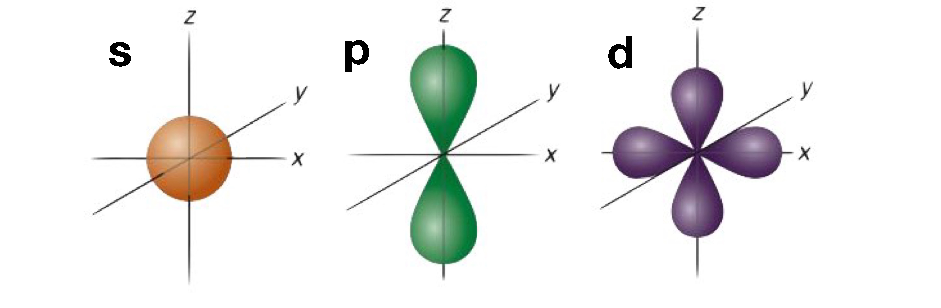
\includegraphics[width=35mm]{src/2_Atoms/images/orbital_shapes.pdf}}
      \end{minipage}
      \begin{minipage}{0.54\linewidth}
        \centerline{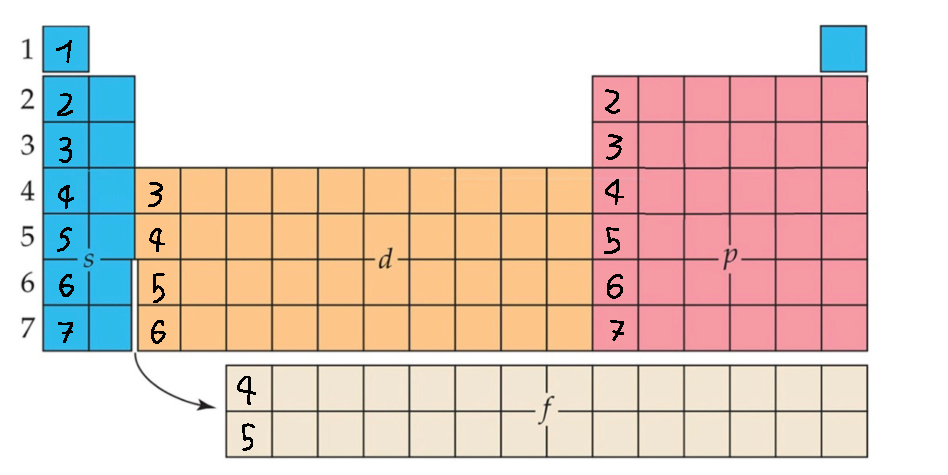
\includegraphics[width=43mm]{src/2_Atoms/images/pse_electron_config.pdf}}
      \end{minipage}
    \end{minipage}
    
    Pauli Exclusion: Each electron has unique set of quantum numbers\\
    Hund's rule: \textbf{Every} orbital in sublevel is first singly occupied\\
    Energy of Hydrogen $e^-$: $E_n = -\frac{hcR_H}{n^2}$, $R_h = 1.097 \cdot 10^7 m^{-1}$\\
    Excitement from shell $n_1$ to $n_2$: $E_H = hcR_H (\frac{1}{n_1^2} - \frac{1}{n_2^2})$

\section{3. Chemical bondings} %Christian
	\subsection{3.1 Covalent bondings}
    Two atoms share electron pairs\\
    \textbf{octet rule:} Atom tries to acquire noble state (2 valence electrons for H and He, 8 valence electrons for all other)\\
    \textbf{exceptions:} 
    \begin{itemize}
        \itemsep0em
        \item Odd electrons
        \item Less / more than 8 VE's on central atom
    \end{itemize}
	\subsection{3.2 Ionic bonding}
    Electrons transfered from atoms with lower EN to atoms with higher EN $\rightarrow$ cations (+) and anions (-).\ electrostatic attraction. $\Delta EN > 1.7 \rightarrow$ ionic bonding\\
    lattice energy $\Delta U$: Energy required to separate ions to infinite distance
	\subsection{3.3 Metallic bonding}
    \begin{minipage}{25mm}
        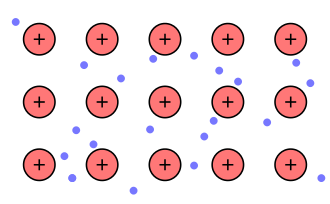
\includegraphics[width=2.5cm]{src/3_Chemical_bondings/images/Metallische Bindung.png}
    \end{minipage}
    \begin{minipage}{42mm}
        cores form grid structure, electron cloud (reason for electricity and heat conduction) surrounds atomic cores
    \end{minipage}
	\subsection{3.4 Polarity and Dipole moment} 
\begin{minipage}{25mm}
    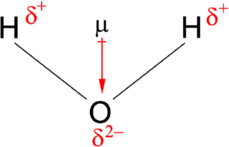
\includegraphics[width=2.2cm]{src/3_Chemical_bondings/images/dipole_moment.png}
\end{minipage}
\begin{minipage}{42mm}
    $\Delta EN>0.5$: polar bonding, density of $e^-$ higher at $\delta^-$ atom.
        If molecular structure leads to  $\rightarrow$ dipole moment exists.
\end{minipage}    


	\subsection{3.5 Formal charges}
    results if new bondings are formed to satisfy octet rule, ignores electronegativity\\
    \textbf{Determine formal charge in Molecule:}
    \begin{itemize}
        \itemsep0em
        \item split all bondings in middle
        \item atoms formal charge = VE if unpaired $- e^-$ of that atom after splitting bondings
        \item effective charge of molecule = sum of formal charges
    \end{itemize}

	\subsection{3.6 Bonding strength and length}
    \begin{tabular}{c c}
        \textbf{length:} $\equiv < = < -$ & \textbf{strength:} $- < = < \equiv$\\
    \end{tabular}
    \vspace*{0.5em}\\
    \textbf{Most stable molecule:}
    \begin{itemize}
        \itemsep0em
        \item least formal charges.
        \item if formal charges necessary: option with the smallest effective charge of molecule
        \item negative formal charge on electronegative atom
    \end{itemize}

\section{4. Molecular models} %Christian
	\centerline{
    \begin{tabular}{c c c c}
        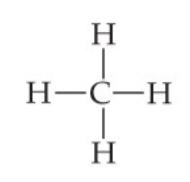
\includegraphics[scale=0.6]{src/4_Molecular_models/images/Structural_formula.png} & 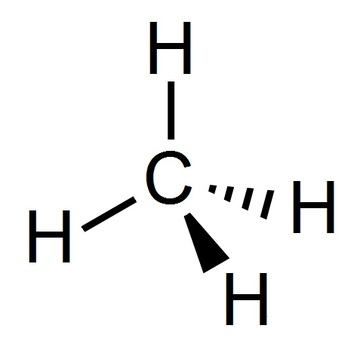
\includegraphics[scale=0.12]{src/4_Molecular_models/images/perspective_drawing.jpg} & 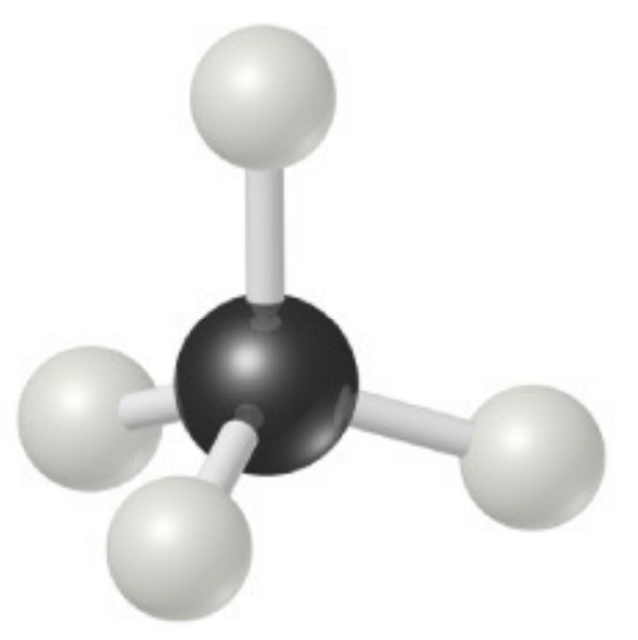
\includegraphics[scale=0.16]{src/4_Molecular_models/images/ball-and-stick_model.png} & 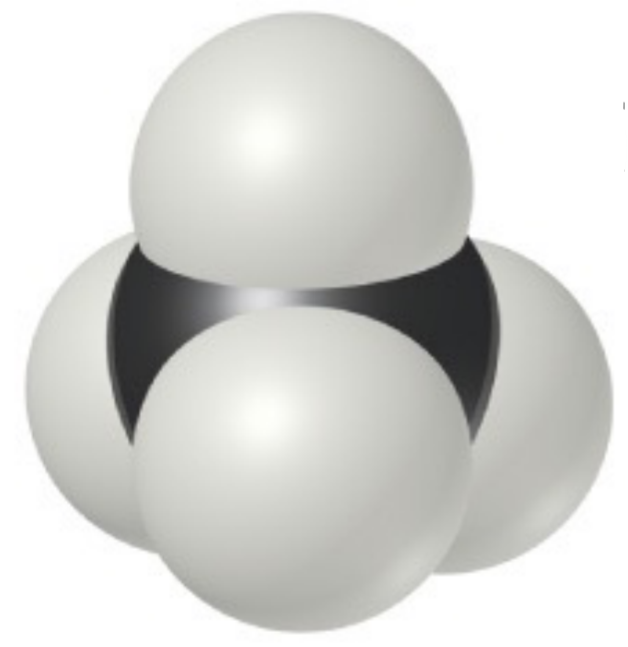
\includegraphics[scale=0.16]{src/4_Molecular_models/images/space-filling_model.png}\\
        structural & perspective & ball-and-stick & space-filling
    \end{tabular}
}
	\subsection{4.1 valence shell electron pair repulsion (VSEPR)}
    \centerline{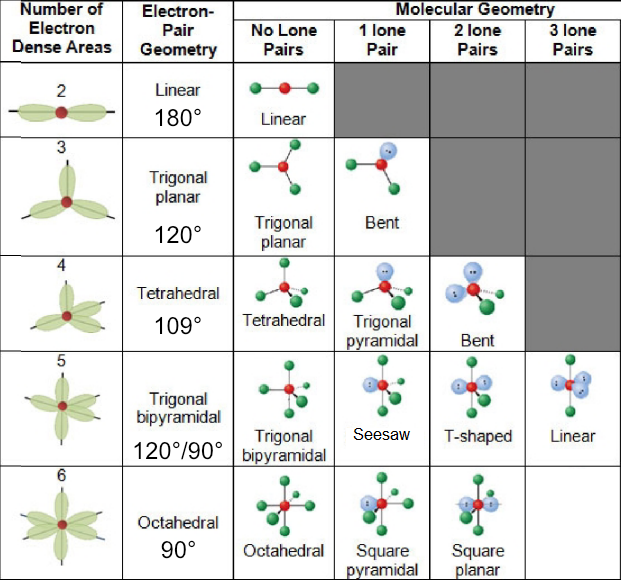
\includegraphics[width=45mm]{src/4_Molecular_models/images/VSPER.PNG}}

\section{5. State of matter} %Noa
	\subsection{5.1 Intermolecular forces}
    \begin{enumerate}
        \item \textbf{Van-der-Waals interactions} (weak)
            \begin{enumerate}
                \item \textbf{Dipol-Dipol} \\
                    Sum of all dipole moments from polar bonds in molecule. (molecular dipole) ($\Delta EN>0.5$)
                \item \textbf{Dispersion} \\
                    Temporary fluctuations of the electrons can cause an induced dipole.
                    \textbf{These forces always exist}. Force increases with molecule size and also affected by molecular shape.
            \end{enumerate}
        \item \textbf{Ion-Dipole Interactions} (strong)\\
            Very important for solutions. Ions solvated by polar liquid.
        \item \textbf{Hydrogen bonding} (strong)\\
            One type of dipole-dipole interaction. N, O, F are very electronegativ $\Rightarrow$ very polar bonds with H.
    \end{enumerate}
    \vspace*{-0.5em}
    \centerline{
        \parbox[t]{1.5cm}{
        \centering
        Ion-Dipole\\$>$ 50kJ/mol}%
        \bm{$>$}
        \parbox[t]{1.5cm}{
        \centering
        H-Bonding\\$\sim$ 25kJ/mol}%
        \bm{$>$}
        \parbox[t]{3cm}{
        \centering
        Dipole-Dipole $\approx$ Dispersion\\$\sim$ 50kJ/mol}%
    }
	\subsection{5.2 Fluids}
    \textbf{Colligative Properties: }Changes depend on amount of solute added, but not which solute.
    $$
    \text{Clausius-Clapeyron} \left\{
        \begin{array}{ll}
            \ln(P_{vap}) = - \frac{\Delta H_{vap}}{RT} + C\\
            \ln(\frac{P_1}{P_2}) = \frac{\Delta H_{vap}}{R} \left( \frac{1}{T_2} - \frac{1}{T_1} \right)
        \end{array}
        \right.
    $$\\*

    % \begin{align*}
    %     \ln(P_{vap}) =& - \frac{\Delta H_{vap}}{RT} + C\\
    %     \ln(\frac{P_1}{P_2}) =& \frac{\Delta H_{vap}}{R} \left( \frac{1}{T_2} - \frac{1}{T_1} \right)
    % \end{align*}

    \textbf{Boiling-Point Elevation:}
    \begin{align*}
        \Delta T_b & = T_b (\textrm{solution}) - T_b (\textrm{solvent}) = iK_b m\\
        m & = \text{molality of solute}\\
        K_b & = \text{molal bp elevation constant (solvent)}\\
        i & = \text{van't Hoff factor}\\
        & = 1 \text{ for non-electrolytes}\\
        & = \text{Number of ions produced for electrolytes.\ e.g 2 for NaCl}
    \end{align*}
    
    \textbf{Vapor-Pressure Lowering: }
        \mathbox{
            P_\text{vap}^\text{sol} = X_\text{solvent} * P_\text{vap}^\text{pure}
        }
    
        Raoult's law $-$ Solution is an ideal solution. All intermolecular interactions are identical.\\

    \textbf{Freezing-Point Depression: }
        \begin{align*}
            \Delta T_f & = T_f (solution) - T_f (solvent) = -iK_{f}m\\
            m & = \text{molality of solute} = (\textrm{moles of solute}) / (\textrm{kg of solvent})\\
            K_f & = \text{molal fp depression constant (solvent)}\\
            i & = \text{van't Hoff factor}
        \end{align*}
	\subsection{5.3 Expressions for Solutions}
\begin{itemize}
    \item $X \; \textrm{Mole fraction} = \frac{\textrm{moles solute or solvent}}{\textrm{total moles}}$
    \item $M \; \textrm{Molarity} = \frac{\textrm{moles solute}}{\textrm{litres solution}}$
    \item $m \; \textrm{Molality} = \frac{\textrm{moles solute}}{\textrm{kg solvent}}$
    \item $\textrm{Mass} \% = \frac{\textrm{mass solute}}{\textrm{total mass}} \cdot 10^2$, ppm: $\cdot 10^6$, ppb: $\cdot 10^9$
\end{itemize}
	\subsection{5.4 Ideal Gas}
    \begin{itemize}
        \itemsep0em
        \item Assumptions of IGL\:
        \begin{itemize}
            \itemsep0em
            \item Gas molecules don't occupy much of total volume.
            \item Gas molecules don't interact.
        \end{itemize}
        \item Ideal Gas Law: $PV = nRT=N kT$
        \item $P\left[Pa\right], V\left[m^3\right], n\left[\text{num of moles}\right], R\left[\frac{J}{mol*K}\right], T\left[K\right]$
        \item Density $\rho = M \cdot \frac{n}{V} = M \cdot \frac{p}{RT}$
    \end{itemize}

    \textbf{Partial pressure:}
    \mathbox{
        P_i=n_i\cdot\frac{RT}{V} \text{ total pressure} =\sum\text{ of all partial pressures.}
    }
    
    \textbf{Henry's law:}\\
    \begin{minipage}{0.99\linewidth}
        \begin{minipage}{0.3\linewidth}
            \vspace*{0.5em}
            \mathbox{
                S_g = k P_g
            }
        \end{minipage}
        \begin{minipage}{0.69\linewidth}
            \begin{align*}
                P_g &= \text{Partial Pressure above liquid}\\
                k &= \text{Henry's law constant}
            \end{align*}
        \end{minipage}
    \end{minipage}
    \vspace*{0.2em}
	\subsection{5.5 Osmotic pressure}
    Pressure needed to counteract osmotic flow.
    \vspace*{-0.2em}
    \mathbox{
        \Pi= i\left(\frac{n}{V}\right) RT=iMRT
    }
    \vspace*{-0.5em}


\section{6. Thermodynamics} %Noa
	\subsection{6.1 System types}
    \begin{itemize}
        \itemsep0em
        \item \textbf{Open} Can echange matter and energy w/ surrounding
        \item \textbf{Closed} Can echange energy w/ surrounding
        \item \textbf{Isolated} Nothing can be exchanged
        \item \textbf{intensive} independent, \textbf{extensive} dependent of system size
    \end{itemize}
	\subsection{6.2 E $=$ Internal energy of system}
    \begin{itemize}
        \item $\Delta E = E_\text{final} - E_\text{initial}$\\
            $\Delta E > 0$ system gained energy\\
            $\Delta E < 0$ system lost energy
        \item \textbf{1st Law of Thermodynamics}\\
            $\Delta E = q + w = q_V$ (constant V)\\ 
            q = heat added to system, w = work done on system
    \end{itemize}
    \vspace*{0.0em}
	\subsection{6.3 Enthalpy, H}
    \vspace*{0.2em}
    $\Delta H$ tells us about heat transferred during chemical reaction.
    \begin{itemize}
        \itemsep0em
        \item $\Delta H = \Delta E + \Delta(PV) = q_p$ heat flow at constant P
        \item $w = -P \Delta V = \text{pressure-volume work} = - \Delta n R T$
        \item $\Delta H > 0 \Rightarrow \text{endothermic}$\\
              $\Delta H < 0 \Rightarrow \text{exothermic}$
    \end{itemize}
	\subsection{6.4 Heat Capacity}
    \vspace*{0.2em}
    Heat flow required to raise substance's T by $1$ degree $^\circ C$ (or $K$)
    \begin{align*}
        C_m & = \text{molar heat capacity} = \left[\frac{J}{mol \; \tccentigrade}\right] = \left[\frac{J}{mol \; K}\right]\\
        C_s & = \text{specific heat capacity} = \left[\frac{J}{g \; \tccentigrade}\right] = \left[\frac{J}{g \; K}\right]\\
        \text{Ex.} \; q & = C_\text{m} \cdot n \cdot \Delta T = C_s \cdot m \cdot \Delta T = \text{ Heat of vaporization}
    \end{align*}
    \textbf{Hess's Law:} $\Delta H_\text{rxn} = \sum \Delta H_i$\\
    e.g Enthalpies of Formation: $\Delta H^\circ_f$
	\subsection{6.5 Entropy, S}
    \vspace*{0.2em}
    Entropy is a measure of disorder in a system. All spontaneous processes are irreversible. S is a state function.
    \begin{itemize}
        \item $\Delta S = \frac{q_\text{rev}}{T}$, $q_\text{rev}$ = heat flow for reversible process
        \item $S = k_b \cdot ln(W)$, $k_b$ = Boltzmann's constant, $W$ = num of microstates
    \end{itemize}
    \bm{$\Delta S > 0$}: increasing microstates\\
    e.g increasing V, increasing T, increasing n, increasing complexity of molecules, melting solids, vaporizing liquids, mixing gases
	\subsection{6.6 2nd Law of Thermodynamics}
    \vspace*{0.2em}
    Entropy of the universe increases for any spontaneous process.
    \begin{align*}
        \Delta S_\text{univ} & = \Delta S_\text{sys} + \Delta S_\text{surr} > 0 \text{ (spontaneous, irreversible)}\\
        \Delta S_\text{univ} & = \Delta S_\text{sys} + \Delta S_\text{surr} < 0 \text{ (nonspontaneous)}\\
        \Delta S_\text{univ} & = \Delta S_\text{sys} + \Delta S_\text{surr} = 0 \text{ (reversible)}
    \end{align*}
	\subsection{6.7 Gibbs Free Energy}
    \mathbox{
        G = H_\text{sys} - T \cdot S_\text{sys} \text{ at constant T}
    }

    % \begin{align*}
    %     \Delta G & < 0 \text{ (spontaneous, irreversible)}\\
    %     \Delta G & > 0 \text{ (nonspontaneous)}\\
    %     \Delta G & = 0 \text{ (reversible)}
    % \end{align*}
    
    \begin{center}
        \begin{tabular}{ |c|c|c|c|c| } 
         \hline
         $\Delta H$ & $\Delta S$ & $-T\Delta S$ & $\Delta G$ & Reaction Characteristics \\ 
         \hline
         - & + & - & - & at all T Spontaneous \\ 
         + & - & + & + & at all T Nonspontaneous \\ 
         - & - & + & +or- & $\downarrow$T Spon.; $\uparrow$T Nonspon.\\
         + & + & - & +or- & $\downarrow$T Nonspon.; $\uparrow$T Spon. \\
         \hline
        \end{tabular}
    \end{center}
    \vspace*{0.5em}

\section{7. Kinetics} %Noa
	\subsection{7.1 Reaction rate}
    \vspace*{0.5em}
    \centerline{Given general rxn: $\alpha A + \beta B \longrightarrow \gamma C + \delta D$}

    \mathbox{
        0 < \text{Rate} = 
        \underbrace{-\frac{1}{\alpha} \frac{d[A]}{d t} = -\frac{1}{\beta} \frac{d[B]}{d t}}_{\parbox[t]{2.4cm}{\centering\footnotesize Rate of disappearance\\of reactants}} = 
        \underbrace{\frac{1}{\gamma} \frac{d[C]}{d t} = \frac{1}{\delta} \frac{d[D]}{d t}}_{\parbox[t]{2.2cm}{\centering\footnotesize Rate of appearance\\of products}}
    }
    \vspace*{-0.5em}
	\subsection{7.2 Rate Law}
    \mathbox{
        \text{Rate} \left[ \frac{M}{s} \right] = k[A]^m [B]^n
    }
    \begin{itemize}
        \itemsep0em
        \item rate only depends on reactants
        \item $k$ is the rate constant
        \item $m,n$ are the reaction orders
        \item $m,n$ can be $0, \frac{1}{2}, 1, 2, \dots$
        \item $m+n$ is overall rxn order
        \item $m,n$ are not necessarily equal to $\alpha, \beta$
    \end{itemize}
    \vspace*{0.0em}
	\subsection{7.3 Reaction Orders}
\vspace*{0.2em}
Consider $A \longrightarrow B$\\
$[A]_t$ = concentration of $A$ at time $t$\\
$[A]_0$ = concentration of $A$ at time $t=0$

\vspace*{-1em}
\begin{minipage}{0.99\linewidth}
    \begin{minipage}{0.65\linewidth}
        \begin{align*}
            \parbox{1.3cm}{\textbf{1st Order}}\\
            \text{Rate} &= -\frac{d[A]}{d t} = k[A]^1 \\
            ln[A]_t &= -k t + ln[A]_0\\
            [A]_t& = [A]_0 \cdot exp(-k t)
            \\[0.5em]
            \parbox{1.3cm}{\textbf{2nd Order}}\\
            \text{Rate} &= -\frac{d[A]}{d t} = k[A]^2 \\
            \frac{1}{[A]_t} &= k t + \frac{1}{[A]_0}
            \\[0.5em]
            \parbox{1.3cm}{\textbf{Zero Order}}\\
            \text{Rate} &= -\frac{d[A]}{d t} = k[A]^0 = k \\
            [A]_t &= -k t + [A]_0 \\
        \end{align*}
    \end{minipage}
    \begin{minipage}{0.34\linewidth}
        \vspace{2.5em}

        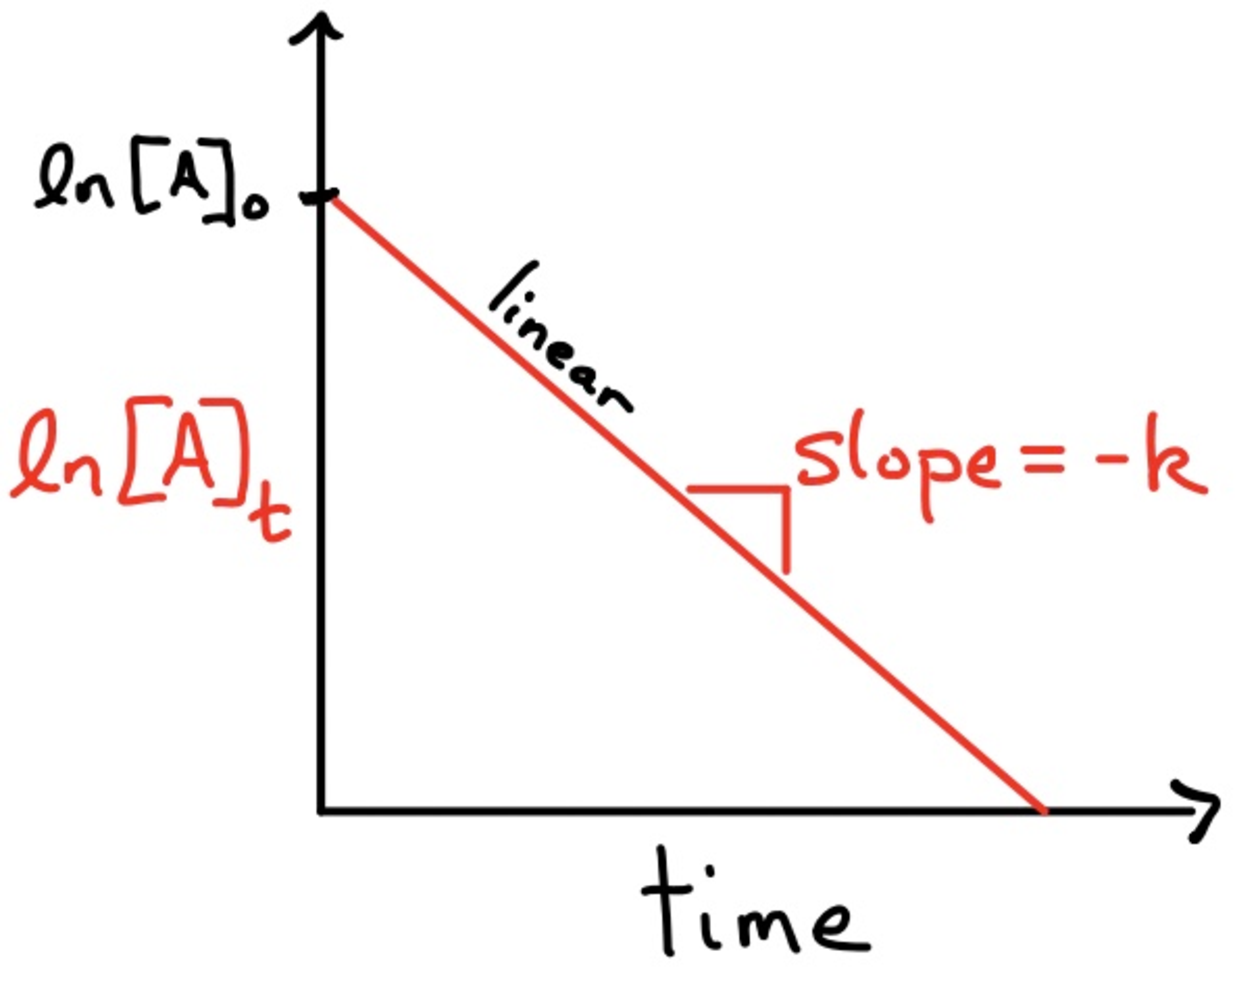
\includegraphics[width=0.9\linewidth]{src/7_Kinetics/images/1st_order.pdf}

        \vspace{0.5em}
        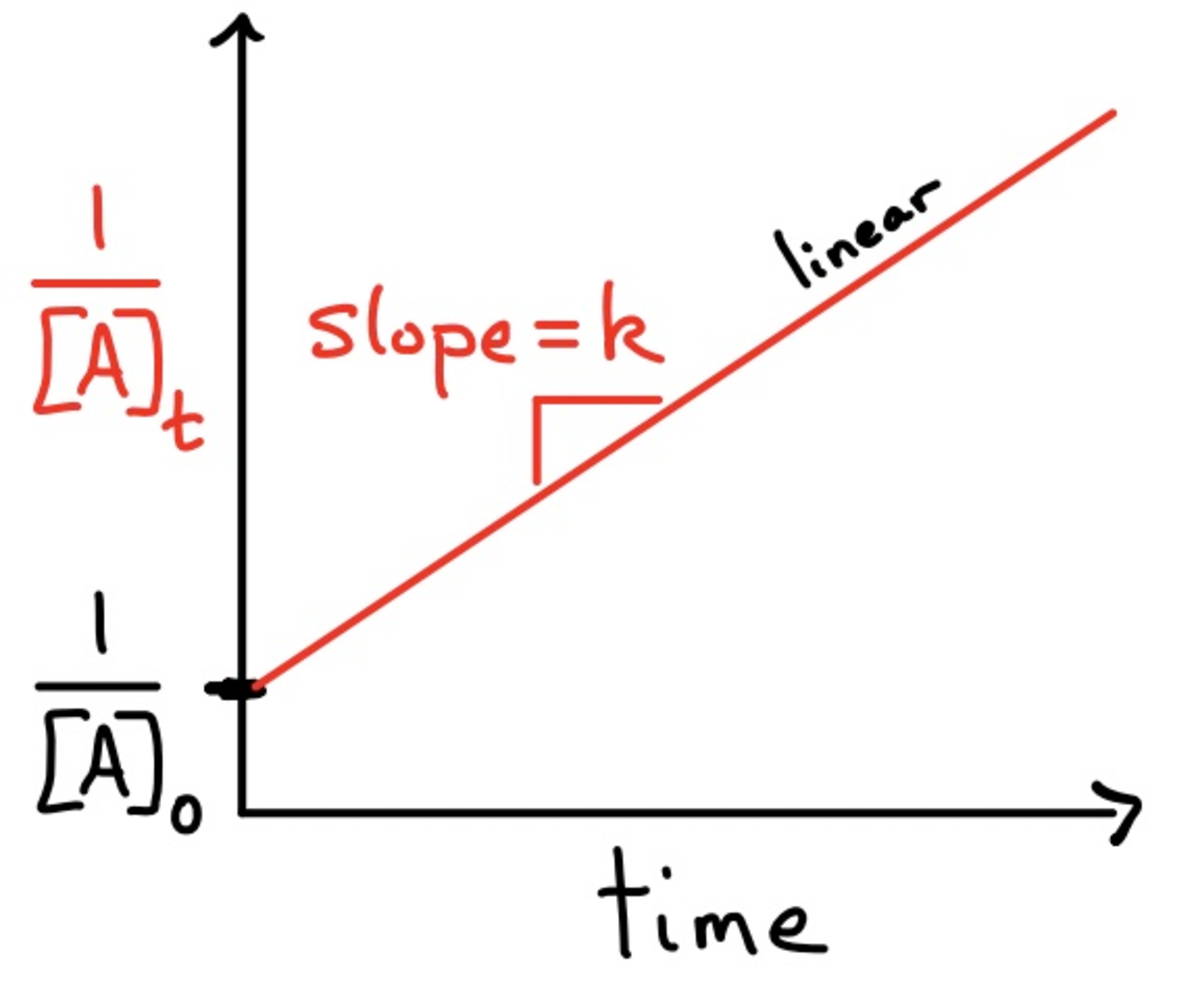
\includegraphics[width=0.9\linewidth]{src/7_Kinetics/images/2nd_order.pdf}

        \vspace{0.5em}
        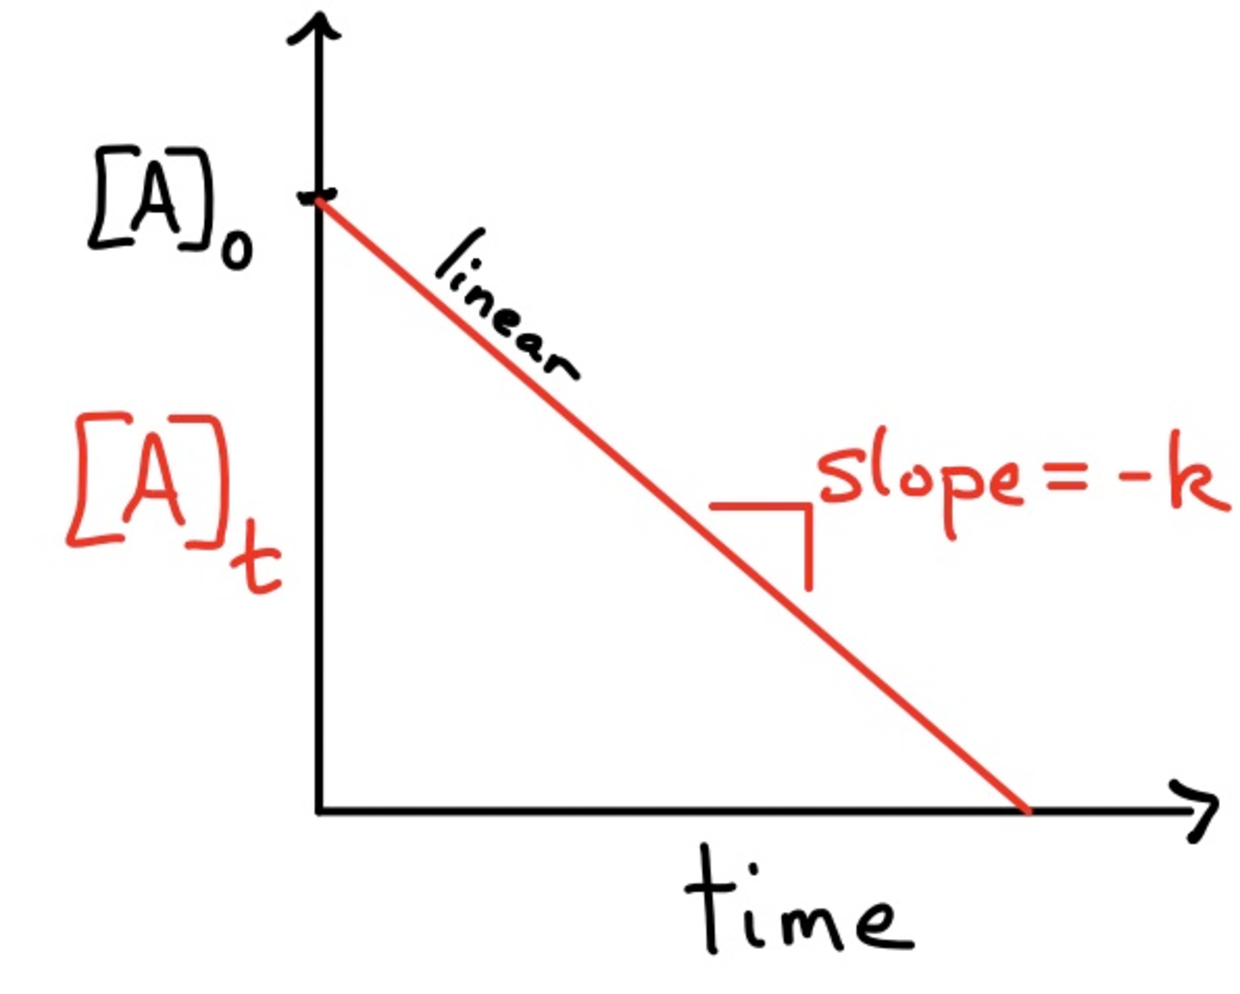
\includegraphics[width=0.9\linewidth]{src/7_Kinetics/images/zero_order.pdf}
    \end{minipage}
\end{minipage}
\vspace*{0.0em}
	\subsection{7.4 Half Life}
    \vspace*{0.0em}
    Time needed for $[A]_t = \frac{1}{2}[A]_0$
    \mathbox{
        \underbrace{\vphantom{\frac{1}{k[A]_0}} t_\frac{1}{2} = \frac{0.693}{k}}_{\textrm{1st Order}} \quad 
        \underbrace{t_\frac{1}{2} = \frac{1}{k[A]_0}}_{\textrm{2nd Order}} \quad 
        \underbrace{\vphantom{\frac{1}{k[A]_0}} t_\frac{1}{2} = \frac{[A]_0}{2 k}}_{\textrm{Zero Order}}
    }
	\subsection{7.5 Collision Model}
    Reaction requires reactant molecules to collide with correct orientation and enough energy.\\
    Higher $T$: reactants collide more often and with more kinetic $E$.\\
    \textbf{Arrhenius}\\
    Molecules need minimum energy to react; Activation Energy, $E_a$\\
    \begin{minipage}{0.99\linewidth}
        \begin{minipage}{0.49\linewidth}
            \centerline{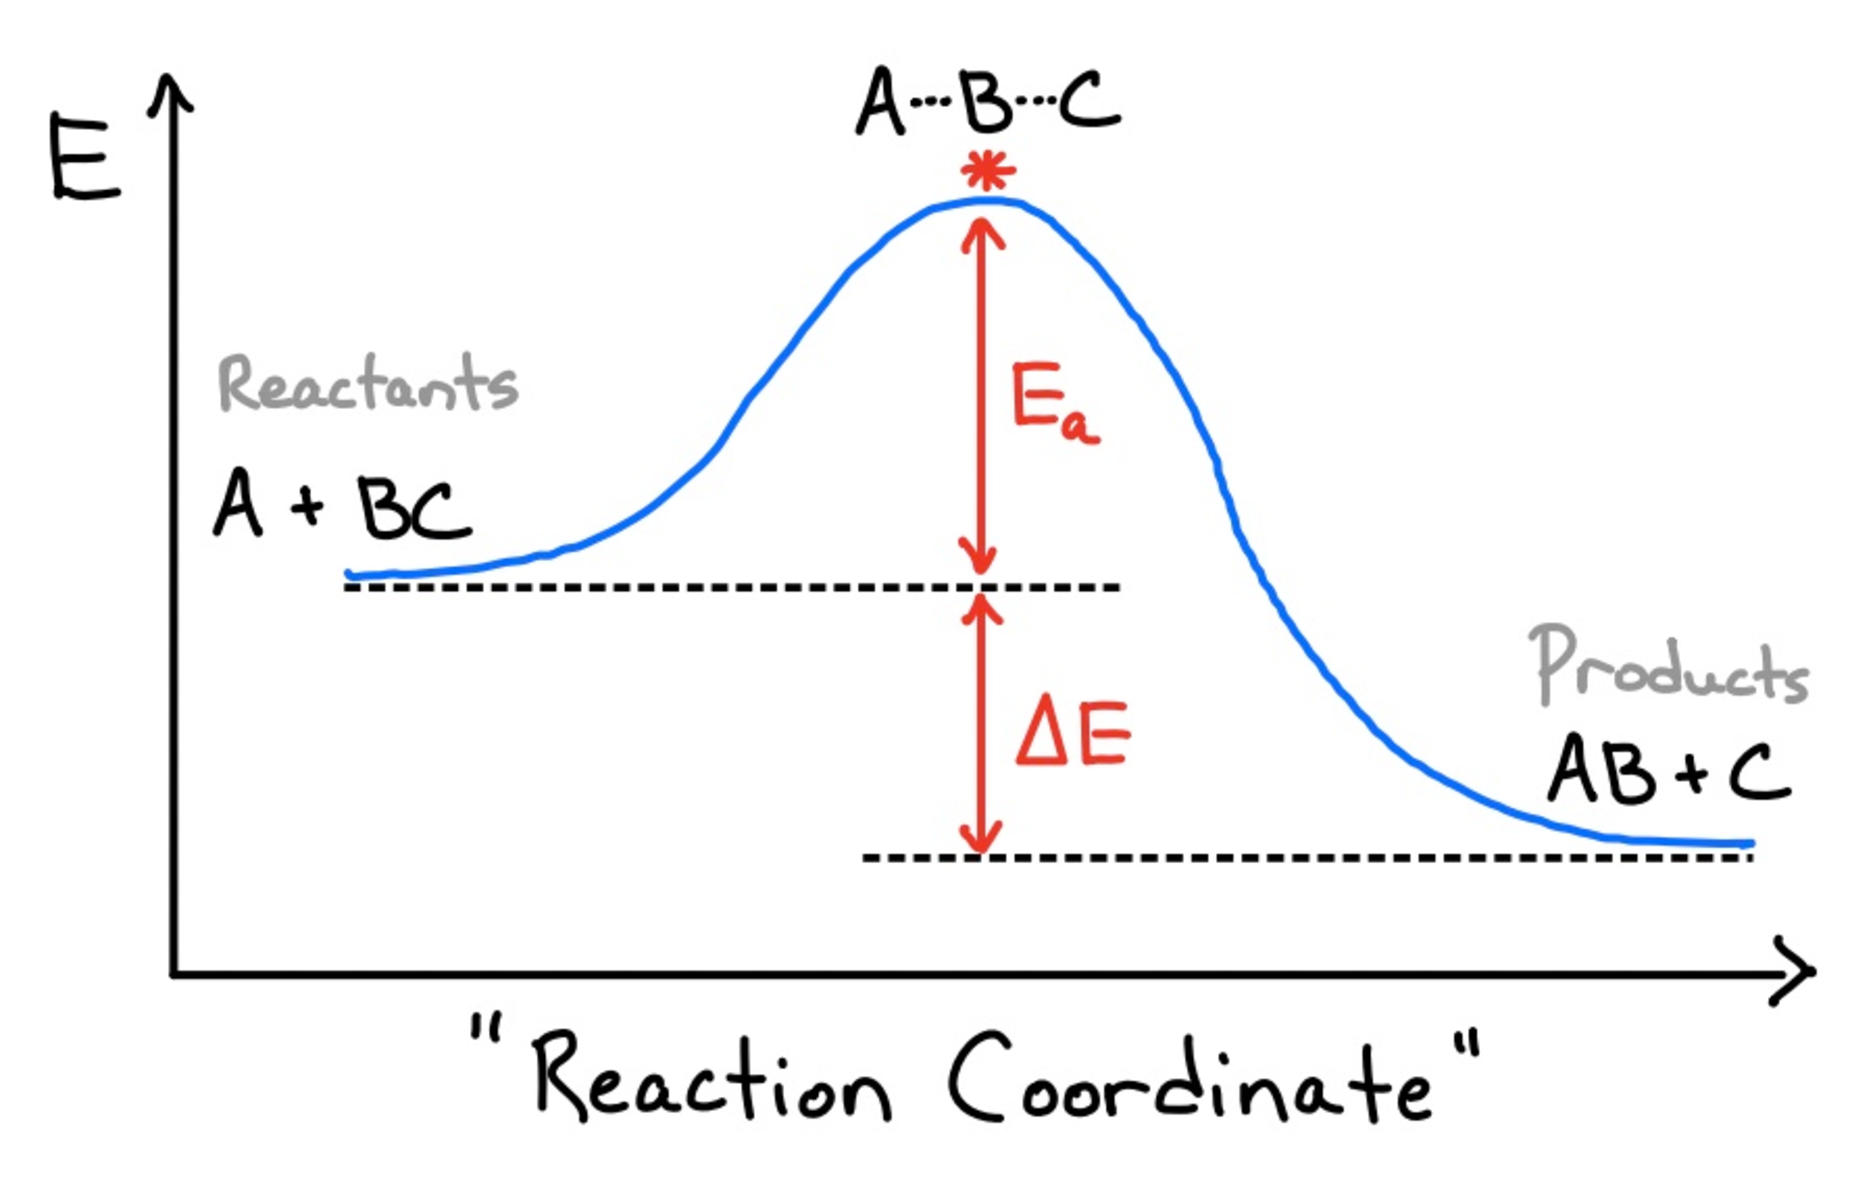
\includegraphics[width=0.8\linewidth]{src/7_Kinetics/images/activation_energy.pdf}}
        \end{minipage}
        \begin{minipage}{0.49\linewidth}
            \centerline{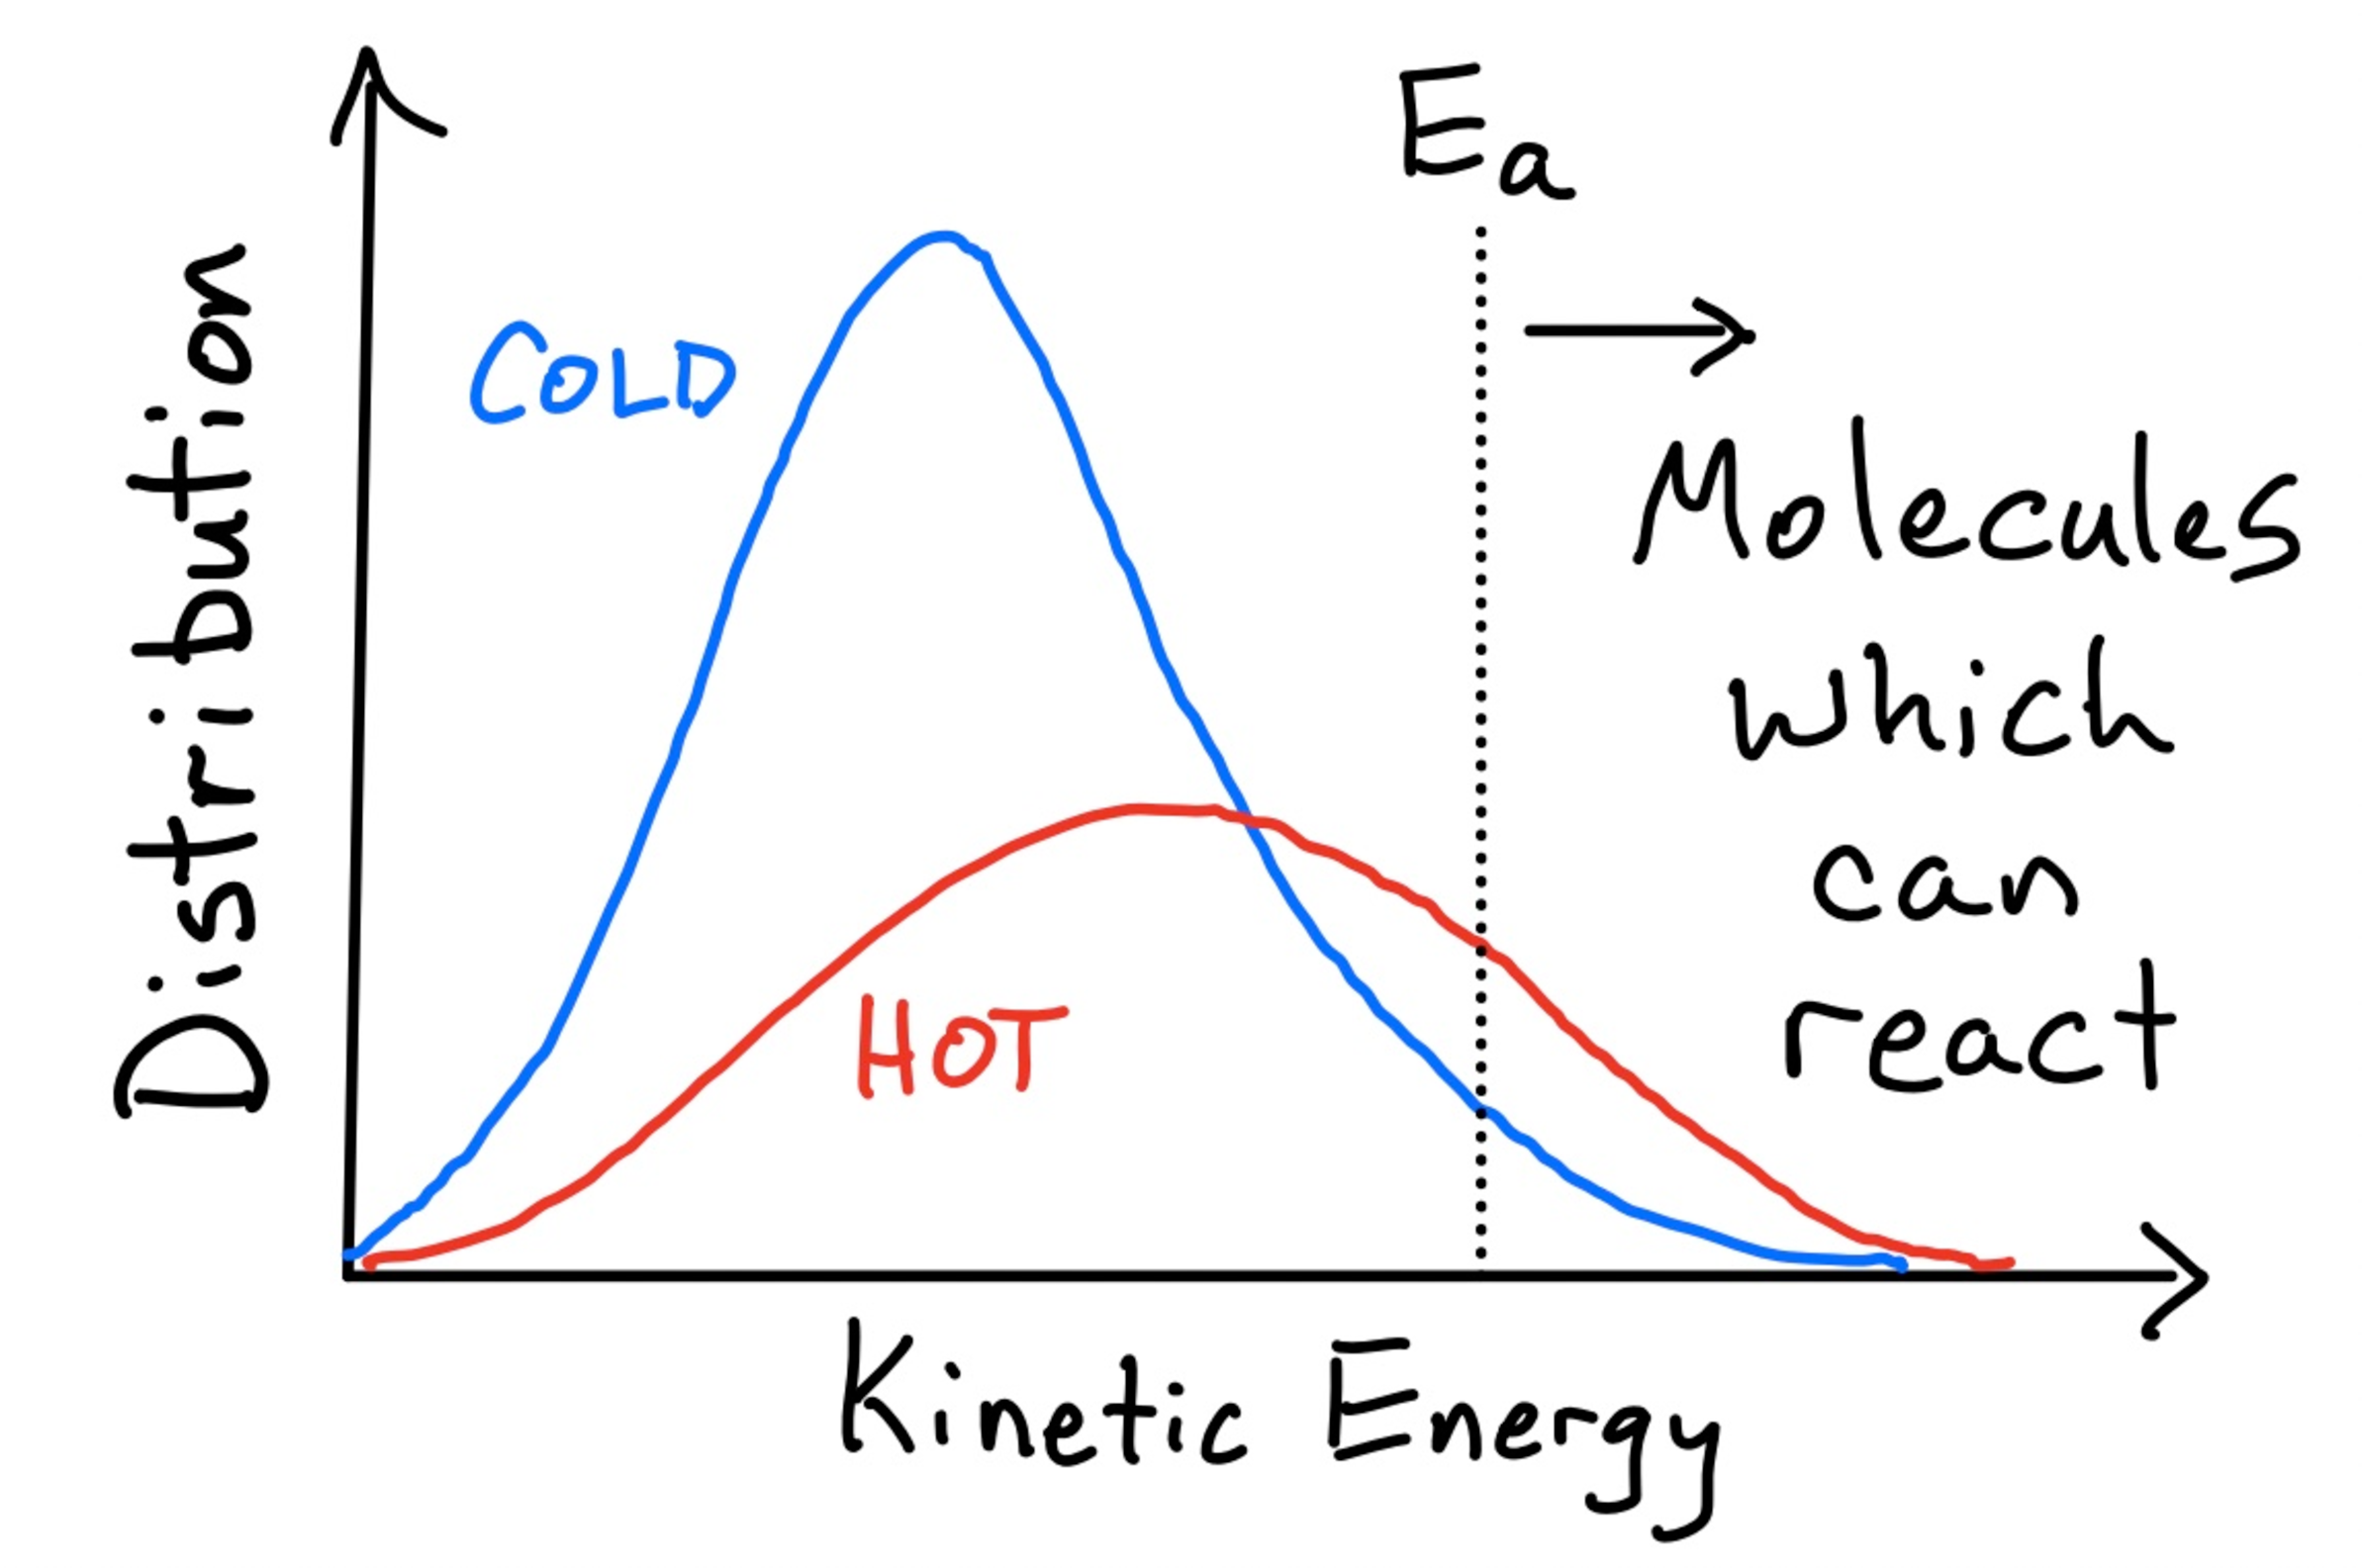
\includegraphics[width=0.8\linewidth]{src/7_Kinetics/images/distribution.pdf}}
        \end{minipage}
    \end{minipage}
    
    
	\subsection{7.6 Arrhenius Equation}
    \vspace*{0.0em}
    \begin{tabular}{c c}
        $\alpha A + \beta B + \gamma C \longrightarrow \text{products}$ & $\text{Rate} = k[A]^m [B]^n [C]^p$
    \end{tabular}

    \mathbox{
        k(T) = \underbrace{(\parbox{0.8cm}{\centering\tiny collisions\\per time})*(\parbox{1.65cm}{\centering\tiny fraction of collisions\\properly oriented})}_{\vphantom{* exp[\frac{-E_a}{R T}]} \parbox{0.8cm}{\centering $A$}}
        * \underbrace{(\parbox{1.7cm}{\centering\tiny fraction of molecules\\with $E>E_a$})}_{\parbox{1.7cm}{\raggedright $*\; exp[\frac{-E_a}{R T}]$}}
    }

    $A$ is a "frequency factor", assumed $T$-independent
    \vspace*{0.5em}

    \begin{minipage}{0.99\linewidth}
        \begin{minipage}{0.49\linewidth}
            \centerline{$ln(k) = \frac{-E_a}{R} \cdot \frac{1}{T} + ln(A)$}
            \vspace*{0.5em}
            \centerline{$\ln(\frac{k_1}{k_2}) = \frac{-E_a}{R} \cdot \left( \frac{1}{T_1} - \frac{1}{T_2} \right)$}
        \end{minipage}
        \begin{minipage}{0.49\linewidth}
            \centerline{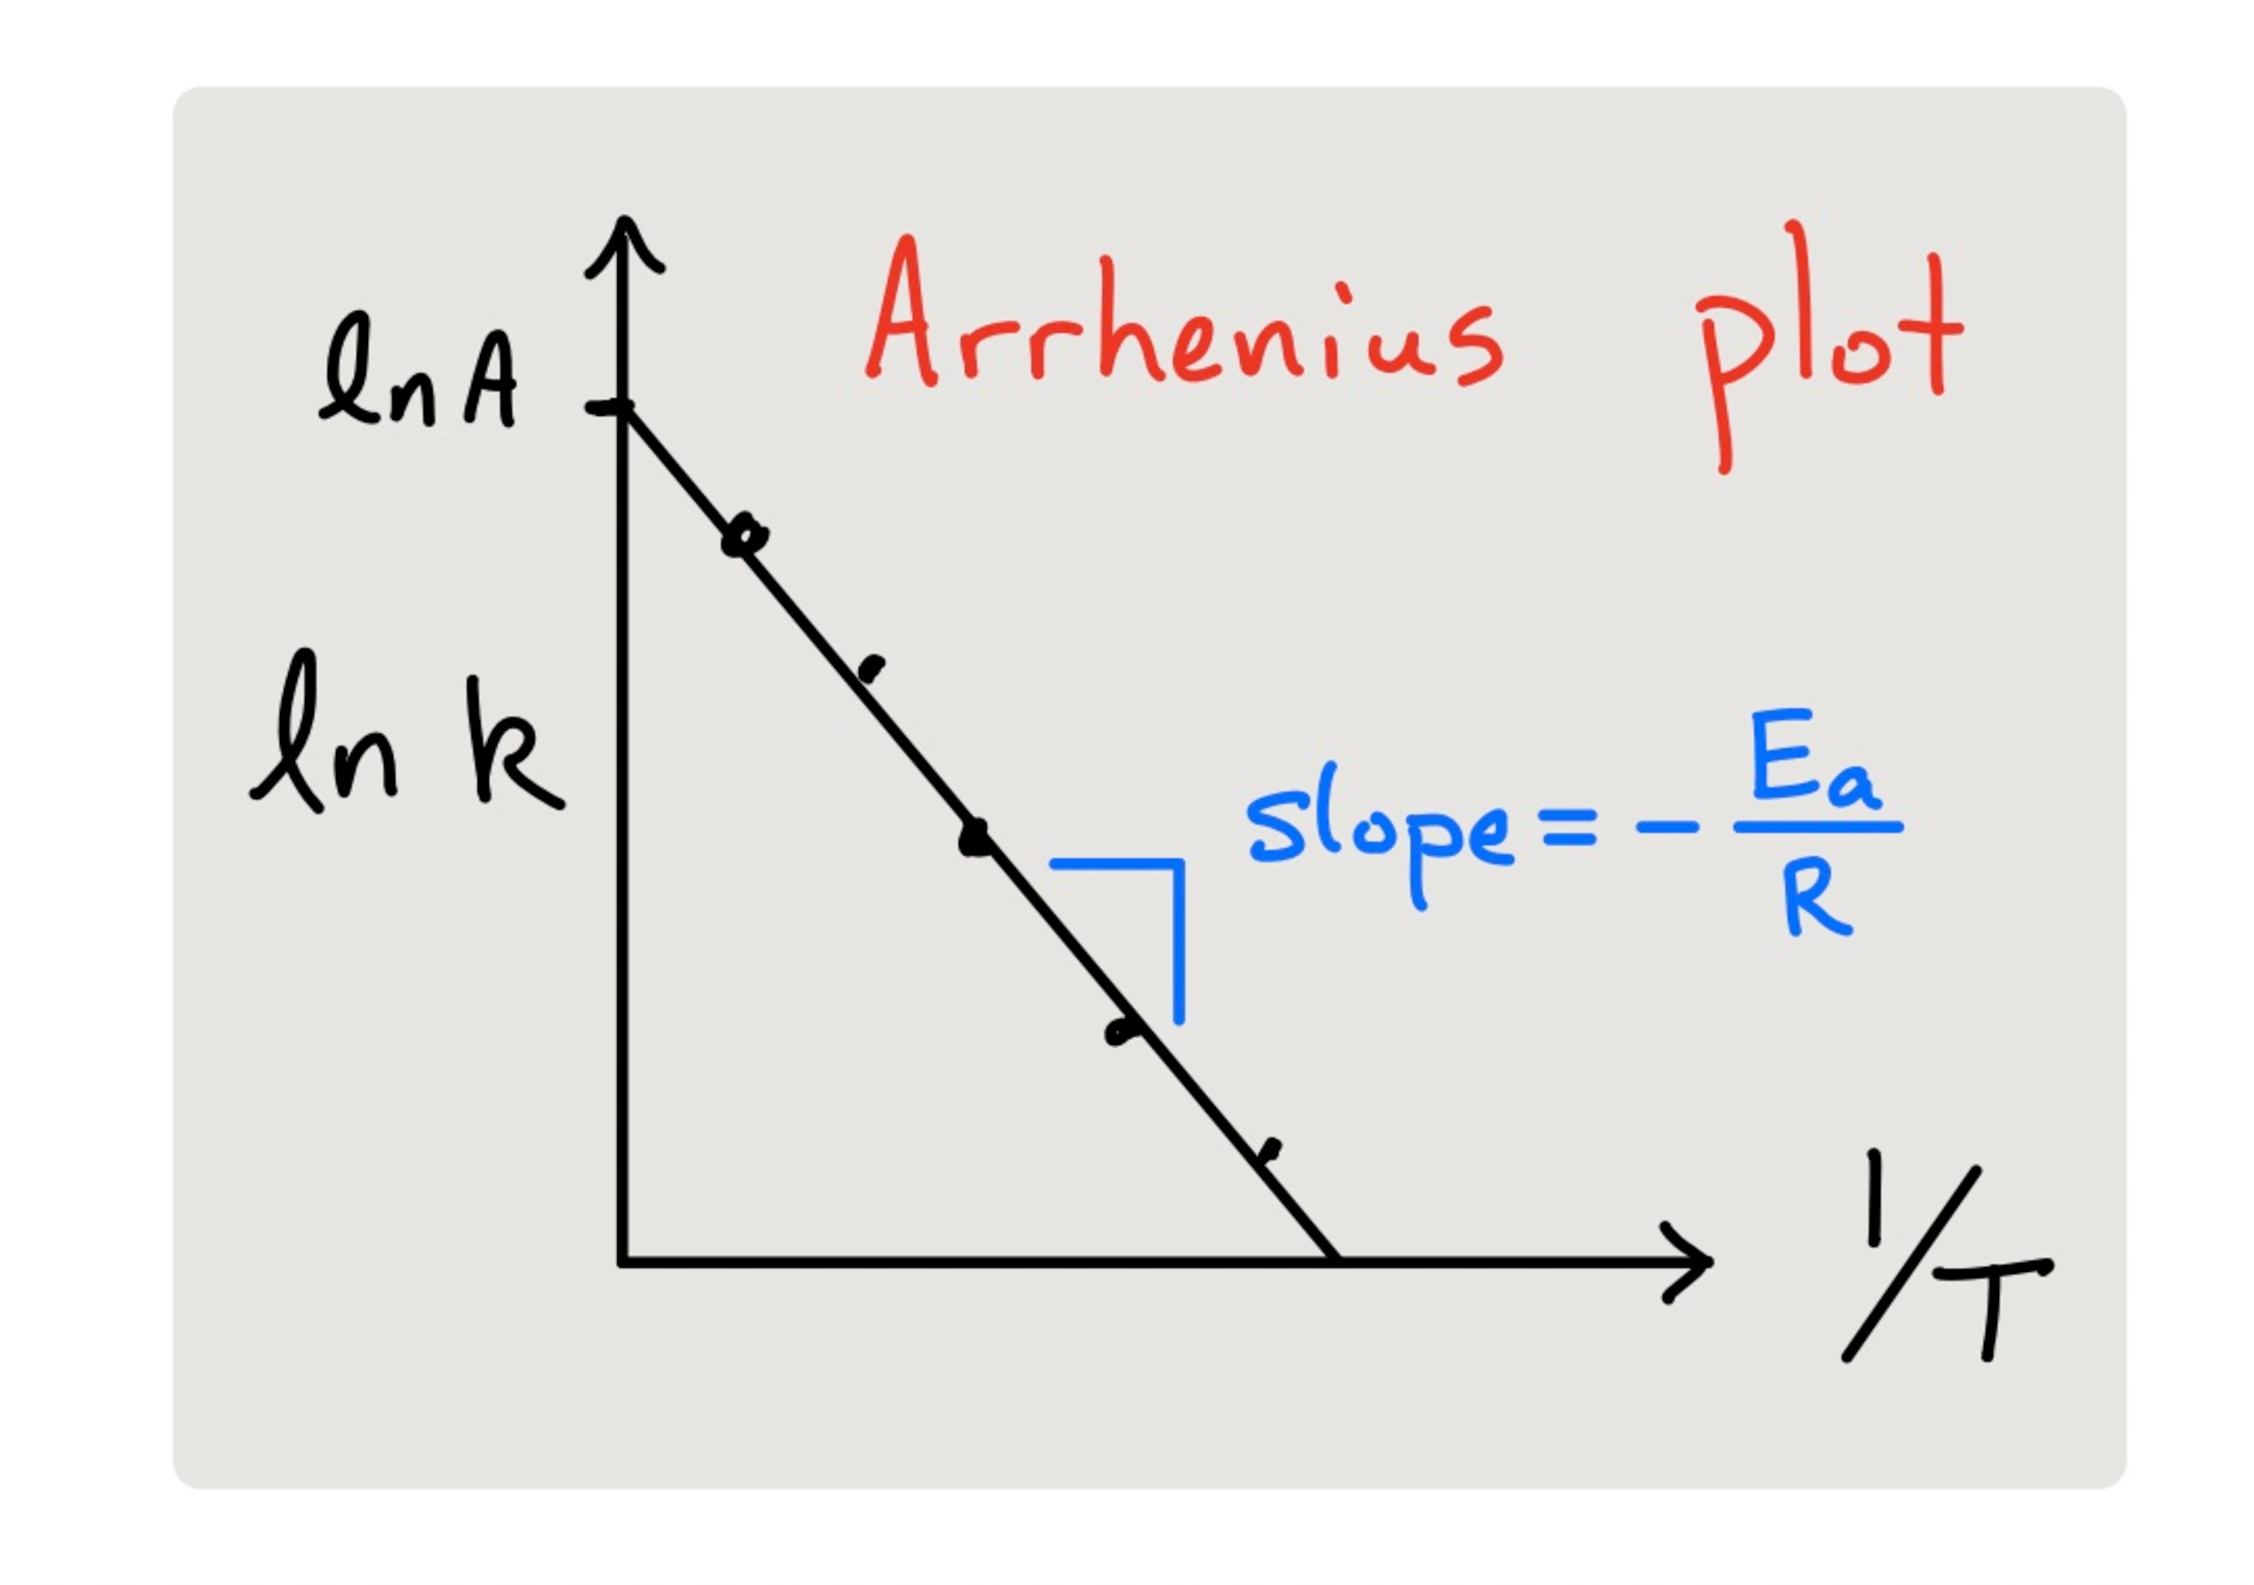
\includegraphics[width=0.8\linewidth]{src/7_Kinetics/images/arrhenius_plot.pdf}}
        \end{minipage}
    \end{minipage}
	\subsection{7.7 Reaction Mechanisms}
    A sequence of elementary rxns that sum to the overall rxn. The kinetics of elementary rxns are determined by
    how many molecules have to collide, referred to as the molecularity.\\
    \columnbreak

    Elementary rxns have rate law where $m,n,p\dots$ are equal to stoichiometric coefficients.
    \vspace*{0.5em}
    
    \begin{center}
        \begin{tabular}{ |c|c|c| } 
         \hline
         \textbf{Molecularity} & \textbf{Elementary rxn} & \textbf{Rate law} \\
         Unimolecular & $A \longrightarrow P$ & $k[A]$ \\
         Bimolecular & $A + A \textrm{ or } A + B \longrightarrow P$ & $k[A]^2$ \\
         Termolecular & $A + A + B \textrm{ or \dots} \longrightarrow P$ & $k[A]^2[B]$ \\
         \hline
        \end{tabular}
    \end{center}
	\subsection{7.8 Multistep Reactions}
    Overall rate law results from the individual rate laws for the individual elementary reactions.
    
    $$
    \left.
        \begin{array}{ll}
            \parbox[t]{0.8cm}{\raggedleft\textrm{2 A}} &\overset{k_1}{\longrightarrow} \; \parbox[t]{1cm}{\textrm{I + C}} \\
            \parbox[t]{0.8cm}{\raggedleft\textrm{I + B}} &\overset{k_2}{\longrightarrow} \; \parbox[t]{1cm}{\textrm{A + D}} \\
            \\
            \hline
        \end{array}
    \right\} \parbox[t]{2cm}{\text{elementary rxns}}
    $$
    $$
    \left.
        \begin{array}{ll}
            \parbox[t]{0.8cm}{\raggedleft\textrm{A + B}} &\overset{}{\longrightarrow} \; \parbox[t]{1cm}{\textrm{C + D}}
        \end{array}
    \right\} \parbox[t]{2cm}{overall rxn}
    \vspace*{0.5em}
    $$
    Assume $k_1 << k_2$, i.e. step 1 is "rate limiting"\\
    $\implies$ rate overall $= k_1[A]^2$
	\subsection{7.9 Catalysts}
    Substances that increase rxn rate, but are neither produced nor consumed in overall rxn.
    $$
    \text{Can} \left\{
        \begin{array}{ll}
            \text{increase A} &\Rightarrow \text{better orient molecules}\\
            \text{lower A} &\Rightarrow \parbox{4cm}{lower energy of transition state or\\allow new mechanism}
        \end{array}
    \right.
    $$
    Lower $E_a$ has bigger impact\\ 
    $\Rightarrow$ Appears in exponent of $k(T) = A*exp(\frac{-E a}{R T})$

\section{8. Chemical Equilibrium} %Christian
	$A \xrightleftharpoons[k_r]{k_f} B$, at equilibrium: Rate $= k_f [A] = k_r[B]$
	\subsection{8.1 Law of mass action, equilibrium-constant}
    \begin{tabular}{c c}
        molarity concentrations & partial pressures\\
        $K_c = \frac{[C]^{\gamma} [D]^{\delta}}{[A]^{\alpha} [B]^{\beta}}$ & $K_p = \frac{[P_C]^{\gamma} [P_D]^{\delta}}{[P_A]^{\alpha} [P_B]^{\beta}} = K_c (RT)^{\Delta n}$
    \end{tabular}
    $K >> 1 \rightarrow$ products dominate, $K << 1 \rightarrow$ reactants dominate
    K depends on T and is unitless\\
    \textbf{heterogeneous equilibria:} exclude pure solids / liquids from K
    reaction quotient $Q$ \textbf{if not at equilibrium}, calculated like $K_c$
    \begin{itemize}
        \itemsep0em
        \item rxn written in reverse: $K = K^{-1}_{\textrm{original}}$
        \item rxn multiplied by n: $K = (K_{\textrm{original}})^n$
        \item multistep rxn: $K = K_1 \cdot K_2 \cdot K_3$ ...
        \item With catalysts: equilibrium is reached faster, K unchanged
    \end{itemize}
	\subsection{8.2 Le Châteliers principle}
    \subsubsection{Disturbance in concentration}
        system reacts to consume added substance
        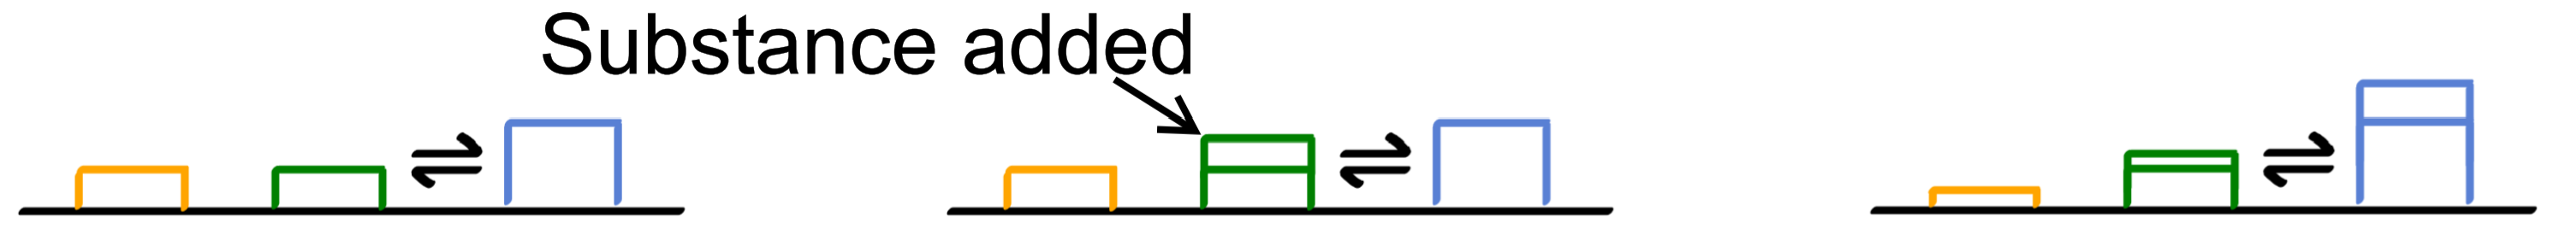
\includegraphics[width=68mm]{src/8_Chemical_Equilibria/images/chatelier_concentration.png}
    \subsubsection{Disturbance in pressure}
        reduced volume $\rightarrow$ system shifts in direction with fewer moles of gas
    \subsubsection{Disturbance in temperature}
        \begin{tabular}{c c c}
             & \textbf{Endothermic} & \textbf{Exothermic}\\
            increased T & right shift & left shift \\
            decreased T & left shift & right shift
        \end{tabular}

\section{9. Acid Base Reactions} %Christian
	\subsection*{9.1 Brownsted Lowry acids and bases}
    \begin{center}$
        \underbrace{HA (aq)}_\text{acid ($H^+$-donor)} + \underbrace{B (aq)}_\text{base ($H^+$-acceptor)} \rightleftharpoons \underbrace{A^- (aq)}_\text{\vphantom{$H^+$} conjugate base} + \underbrace{HB^+ (aq)}_\text{\vphantom{$H^+$} conjugate acid}
    $\end{center}
    strong acids/bases completely ionize, weak acids/bases don't
    \vspace*{0.0em}
	\subsection{9.2 Autoionisation of water}
    Amphiprotic substances (ex. Water) can act as acid \textbf{and} base
    \begin{gather*}
        \underbrace{H_2O(l)}_\text{acid} + \underbrace{H_2O(l)}_\text{base} \rightleftharpoons \underbrace{OH^- (aq)}_\text{conjugate base} + \underbrace{H_3O^+ (aq)}_\text{conjugate acid}\\
        K_w \equiv K_C = [OH^-][H_3O+] = 10^{-14} (25\textrm{°}C)
    \end{gather*}
    
	\subsection{9.3 Reaction of acid with water / base with water}
    \begin{tabular}{c c}
        acid-dissociation & base-dissociation\\
        $K_a \equiv K_C = \frac{[A^-] [H_3O^+]}{[HA]}$ & $K_b \equiv K_C = \frac{[HB^+] [OH^-]}{[B]}$
    \end{tabular}
	\subsection{9.4 p-Scales}
\vspace*{-0.5em}
    \begin{center}
        \begin{tabular}{c c c}

        \end{tabular}
        \begin{minipage}{0.99\linewidth}
            \begin{minipage}{0.31\linewidth}
                \center
                $p(\xi) = \mbox{-}\log(\xi)$\\
                $pH + pOH = 14$
            \end{minipage}
            \begin{minipage}{0.34\linewidth}
                \center
                $pH = \mbox{-}\log[H_3O^+]$\\
                $pH < 7 \rightarrow$ acid
            \end{minipage}
            \begin{minipage}{0.33\linewidth}
                \center
                $pOH = \mbox{-}\log[OH^-]$\\
                $pH > 7 \rightarrow$ base
            \end{minipage}
        \end{minipage}
    \end{center}
	\subsection{9.5 common ion effect and Buffers}
    $CH_3COOH + CH_3COONa \rightarrow$ dissociates to $CH_3COO^-$
    \begin{gather*}
        HA(aq) + OH^-(aq) \rightleftharpoons A^-(aq) + H_2O(l)\\
        A^-(aq) + H_3O^+(aq) \rightleftharpoons HA(aq) + H_2O(l)\\
        [H_3O^+] = K_a \frac{[HA]}{[A^-]} \rightarrow pH_{\textrm{buffer}} = pK_a + \log \left( \frac{[base]}{[acid]} \right)
    \end{gather*}
    \vspace*{-0.5em}
    For disturbance small relative to $[HA],[A^-] \rightarrow$ small pH change\\

\section{10. Redox Reactions} %Noa
	\subsection{10.1 Oxidation Numbers}
    \begin{itemize}
        \itemsep0em
        \item Atoms in elemtal form: \textbf{0}
        \item Monoatmic ions: \textbf{ionic charge}
        \item Nonmetals in ionic/molecular compounds:\\ \textbf{negative oxidation numbers}\\
            \begin{tabular}{l l}
                Oxygen: \textbf{-2} & (except peroxide ion, $O_2^2-$, \textbf{-1})\\
                H: \textbf{+1} & (except if bonded to metal, \textbf{-1})\\
                F: \textbf{-1} & (always)\\
                Cl, Br, I: \textbf{-1} & (except if bonded to oxygen)
            \end{tabular}
        \item Sum of oxidation numbers for atoms in compound equals its net charge
    \end{itemize}
	\subsection{10.2 Energy and Batteries}
    \begin{minipage}{34mm}
        \begin{itemize}
            \itemsep0em
            \item Cathode \textcircled{+}: reduction
            \item Anions $\rightarrow$ anode
        \end{itemize}
    \end{minipage}
    \begin{minipage}{31mm}
        \begin{itemize}
            \itemsep0em
            \item Anode \textcircled{-}: oxidation
            \item Cations $\rightarrow$ cathode
        \end{itemize}
    \end{minipage}
    \vspace*{0.5em}

    Electric potential = potential energy difference per unit charge
    \begin{align*}
        1V =& \frac{1.6 \cdot 10^-19 J}{1.6 \cdot 10^-19 C}\\
        E^\circ_\text{cell} \equiv& \; \text{Cell voltage at standard conditions}\\
        E^\circ_\text{red} \equiv& \; \text{Potential energy available if reduced}\\
        \text{Cell potential} \Rightarrow E^\circ_\text{cell} =& \; E^\circ_\text{red}(\text{cathode}) - E^\circ_\text{red}(\text{anode})
    \end{align*}
	\subsection{10.3 Connection to Gibbs Free Energy}
\vspace*{-0.5em}
    \begin{minipage}{0.99\linewidth}
        \begin{minipage}{0.32\linewidth}
            \centerline{$\Delta G^\circ = -n F E^\circ_\text{cell}$}
            \vspace*{2em}
            \centerline{$E^\circ_\text{cell} > 0, \Delta G^\circ < 0$}
            \vspace*{0.5em}
            \centerline{$\Rightarrow \textbf{Spontaneous!}$}
        \end{minipage}
        \begin{minipage}{0.61\linewidth}
            \begin{align*}
                \Delta G^\circ =& \; \textrm{J/mol of rxn}\\
                F =& \; \textrm{Faraday's constant}\\
                n =& \; \textrm{unitless number moles of} \; e^- \textrm{'s}\\
                & \; \textrm{transferred in balanced cell rxn}\\
            \end{align*}
        \end{minipage}
    \end{minipage}

\end{document}